\documentclass{article}

\usepackage{preamble}

\usepackage[style=numeric]{biblatex}
\addbibresource{kasper_speciale_2017.bib}

%\title{Transmembrane protein prediction using long short-term memory networks}
%\author{Kasper Lynderup Jensen}
%\date{\today}

\begin{document}

%\maketitle

\begin{titlepage}
	\centering
	{\scshape\LARGE Aarhus University \par}
	\vspace{1cm}
	{\huge\bfseries Transmembrane Protein Prediction using Long Short-Term Memory Networks\par}
	\vspace{2cm}
	{\Large\itshape Kasper Lynderup Jensen \par}
	\vfill
	Supervised by\par
	Christian Storm Pedersen
	
	\vfill
	
	% Bottom of the page
	{\large \today\par}
\end{titlepage}

\section*{Abstract}
Transmembrane Protein Prediction is a problem with many uses 
as experimental determination of protein structures is still expensive
and for different purposes it can be useful to know the structure.
Here I introduce a small long short-term memory network based model 
which gives a precision of $67 \pm 3$ and a recall of $71 \pm 3$. 
The model manages, when compared to TMSEG \cite{tmseg}, slightly 
worse but is still a lot better than a simple Hidden Markov Model.

\tableofcontents

% Introducere trans membrane proteiner. hvordan er de representeret, en streng af amino syre
% Forskellige dele af proteinerne har forskellige fordelinger af aminosyre. Dette kan benyttes af en computer
% Introducere trans membrane protein helix prediction, et problem der muligvis kan løses med machine learning
\section{Introduction}
% Introducere trans membrane proteiner. hvordan er de representeret, en streng af amino syre
% Forskellige dele af proteinerne har forskellige fordelinger af aminosyre. Dette kan benyttes af en computer
% Introducere trans membrane protein helix prediction, et problem der muligvis kan løses med machine learning

% motivation: Inden for andre fields er nogle af de bedste løsninger med LSTMs. Vi vil se om man kan bruge LSTMs til TMprediction.
% inspiration: TMSEG

\glspl{tmp} is a kind of proteins that crosses the membrane, they have an important
role in many living organisms \cite{heijne} and different areas is interested in theirs structure,
among other as drug targets \cite{OveringtonEtAl}, but it can be expensive to experimental determine 
their structure, and it could therefore be beneficial if it was possible to determine
the structure from the protein's composition. This is the problem of \gls{tmp} prediction.
Instances in this problem comes as a string of characters corresponding to the sequence 
of amino acids the protein consists of. The goal is then to predict the structure 
from this sequence. The structure consists of three parts, the parts of the protein 
that goes through the membrane, called \glspl{tmh}, the part that is inside, and the part 
that is outside. The structure is represented as a string the same length as the 
amino acid sequence and consists of different characters corresponding to which part
of the structure, the amino acid at the same position belong to.
This is possible because the distribution of amino acids is different in the different 
parts. This distribution or pattern can be approximated by training a machine learning 
model. The training is done by showing the model examples of \glspl{tmp} with known
structure.

Here I will build a machine learning model to try to solve this problem. The model
will be based on the model TMSEG \cite{tmseg}, it will use different machine learning
methods but will follow TMSEG in both how the problem is approached and how the result
is measured. Most traditional machine learning approaches needs a lot of knowledge 
about the problem to be able to extract the relevant information from the input data.
Here i will examine the possibility of skipping this step by feeding the raw input 
into the model, this I have done by basing the model on a type of \glspl{rnn} called 
\glspl{lstm}. \glspl{lstm} have had a lot of success in other areas and here I will 
examine their suitability in this problem. I will run a number of experiments to determine
how this model compares with other models. 

% Hvad har andre folk gjort med problemet, nævn nogle stykker og forklar hvad de har gjort
% Slut af med tmseg og beskrev hvad de har gjort mere beskrivende.
% Hvad har andre folk gjort med machine learning problemer baseret på sekvens data
\section{Related work}
\subsection{Transmembrane Protein Prediction}
% "A hidden Markov model for predicting transmembrane helices in protein sequences"\cite{tmhmm} fra bioinformatik-kurset. 
		% At TM prediction er muligt og kan gøres "simpelt" med HMM
% 
% i TMSEG nævnes MEMSAT. måske skal vi skrive noget om den

% Der var en artikel der hedder HTP der virker interressant

% Hvilke modeller eksisterer allerede og bliver brugt pt. 

\subsection{Long Short-Term Memory Networks}
%Find nogle artikler der laver noget nice med lstm

A lot af recent exiting advances in areas where the data is inherently sequence based 
have been done with \gls{lstms}. Areas such as language modelling \cite{JozefowiczEtAl, ShazeerEtAl},
speech recognition \cite{XiongEtAl}, machine translation \cite{WuEtAl} and many more, have had the 
state of the art moved by the use of \gls{lstms}. 



% Beskriv nn. brug nn's problemer til at indroducere rnn
% Beskriv rnn. brug rnn's problemer til at indroducere lstm
% Beskriv lstm
\section{Theory} %\todo{Different name!}
% Beskriv nn. brug nn's problemer til at indroducere rnn
% Beskriv rnn. brug rnn's problemer til at indroducere lstm
% Beskriv lstm

% Hvad er neural network, recurrent nn, lstm
% Tegning/diagram over de forskellige ting - husk at det skal være relevant og skarpt.

\subsection{Neural Network}
% feed forward networks bruges bl.a. til image-recognition	
		
An \gls{ann} is a function that maps an input vector to an output vector. 
It is consisting of layers interacting in some way. A typical \gls{ann} is the \gls{mlp}.
It consists of multiple layers were each layer uses the last layer's output as input.
The combutation that each layer does is multiplying it's input with a weight, adds a bias and applies 
some non-linear activation function. As a function, a \gls{mlp} can be written as:

\begin{align*}
	MLP(x) &= MLP_L(x) \\
	MLP_l(x) &= f(W_l * MLP_{l-1} + b_l) \\
	MLP_0(x) &= x
\end{align*}

where $w_l$ is a weight matrix, $b_l$ is a bias vector and $L$ is the number of layers after the 
input layer, if $L=2$ it is a shallow network with only one hidden layer and if greater it is a deep network
with multiple hidden layers.

The \gls{mlp} is multiplying the input by some weight matrix that cannot change dimensions from input to 
input, it therefore requires that the input have some fixed length. This can give difficulties with 
problems where instances is sequences of different lengths. Different techniques, each with it's own 
shortcomings, can be used to apply \glspl{mlp} in such areas. 
Two typical ways to do this is with a sliding window or with some sort of feature extraction or 
a combination of the two. If the wanted output for the sequence is fixed length, like a classification, 
% TODO like in tmseg step3, "is the seqment a tmh or not
one can transform the input sequence to some fixed length by extracting the most important information
from it. A problem with this is that some information has to be discarded and it is not always 
obvious to see which features is the important ones, this usually require export knowledge in the
field from with the problem originates. 
If the wanted ouput is on the other hand a sequence, a sliding window can be used. 
This is done by taking a fixed length segment of the sequence and using that as input to compute 
a fixed length segment of the output and then moving the window by some amount in the sequence and compute 
a new segment of the output, this is then repeated until the window has sled through the whole sequence.
An advantage with this technique is no information is thrown away, but if some part of the output is 
dependent on different parts of the input, it can be hard to chose a window length that 
encapsulate all part of the input that it depends on, this can be remedied by augmenting 
the window with features extracted from the whole sequence, but this involve the same problems 
from before.

	
\subsection{Recurrent Neural Network}
% \cite{rnnLTD} pointere problemer med rnn

% Recurrent neural network: keyword = recurrent
% kan ikke "huske", hvad der tidligere er set.


\subsection{Long Short-Term Memory Network}
% \cite{lstm} introducere lstm som løsning til ovenfor

% lstm's:
% Indeholder en CellState = LONG short-term memory
% Det er stadig bare en matematisk beregning
% DEN MATEMATISKE BEREGNING
% vi kan benytte det til at kigge på proteinstrenge! yearh!

% Hvordan har vi valgt at prøve at løse problemet.
% Vi har delt problemet op i subproblemer ligesom tmseg
% Vi har prøvet at bruge andre machine learning metoder
% Største forskel er at vi har givet model "rå" data i stedet for feature extraction
% Fordelen er at man ikke behøver at på forhånd finde ud af hvilke features er vigtig

% Hvilke muligheder er der for at implementere modelen. forskellige ml libraries
% Vi har valgt tensorflow
\section{Model}
% Hvordan har vi valgt at prøve at løse problemet.
% Vi har delt problemet op i subproblemer ligesom tmseg
% Vi har prøvet at bruge andre machine learning metoder
% Største forskel er at vi har givet model "rå" data i stedet for feature extraction
% Fordelen er at man ikke behøver at på forhånd finde ud af hvilke features er vigtig

% Hvilke muligheder er der for at implementere modelen. forskellige ml libraries
% Vi har valgt tensorflow

% Noget om hvorfor lstm
	% Der er flere beregninger når man bruger lstms (con)
	% Long short-term memory: Hvorfor har vi brug for LONG memory?
% Hvad gør vores model forskelligt fra tmseg

% Hvad forventer vi vores model kan gøre bedre end de modeller der allerede eksisterer?

% tegning af model!!

%  Problem delt op i 4 steps som i tmseg
% Kun 3 af stepsne er machine learning
	% Første step assigner en sandsynlighed for hver klasse til hver position i sekvens
		% Vi har gjort det med en lstm, fodret med den rå sekvens
		% Første lag embeder sekvens data i et vector rum
		% Andet lag er en bidirectionel lstm 
		% Trejde og sidste lag er et softmax layer som giver en sansynligheds fordeling af de forskellige klasser
		
	% Andet step er at give hver position en klasse ud fra dens sandsynlighed 
		% med forbehold for at helixer ikke må være for korte
		% Måske tilføje et bias til nogle af klasserne
		% Ikke machine learning men mere post processing af af første step
		
	% Trejde step er justering af enderne af helixerne
	
	% Fjerne step er finde en topologi af sekvens, 
		% ie hvilken vej vender helixerne og hvilke dele er inden for membranen og hvilke er uden for

In many \gls{ann} based models it is very hard to ensure some syntax rules for the output. If the output 
classes was \gls{tmh}, inside and outside, then it should not be possible for a output sequence to contain 
adjacent positions with one being inside and the other being outside or both ends of a \gls{tmh} to be on the 
same side, but these rules cannot be ensured. If the problem is devided in sub problems in such a way that 
the rules is in the way the problem is divided. 

\subsection{Machine Learning Libraries}

\subsection{Implementation}
% Hvorfor tensorflow, python
% Hvad får vi fra tensorflow, hvilket arbejde har vi selv gjort
% Hvor meget arbejde ligger der i de forskellige dele af model

% Tensorflow giver selve machine learning bygge klodserne 
% men vi har selv sat dem sammen til en model 
% For og efter behandling af dataen har der også lagt meget arbejde i

% Beskriv alle experimenter vi har kørt
\section{Experiments}
% which experiements will we do on our model?
	% List them - gør det overskueligt!!!
	
% Hvad vil det sige at predicte en helix
% Skal hver position have den rigtige klasse
% Skal den ses som et samlet strykke af positioner med samme klasse.
% i så fald hvornår er den rigtig.
% Vi har brugt to forskellige mål for hvornår en prediction er rigtig
% Den første kræver 50% overlap og ender inden for 5 position for at den gælder som rigtig
% Den anden kræver kun 25% overlap

	
% The results we allready have of the other model - or the tests we need to do, to be able to compare the models.
% the data used

% Hvad forventer vi resultaterne vil være.

All the weights and biases in the model gets initialized by random values and the training
is done by mini-batch gradient descent, where a random batch of the samples is used to 
calculate the gradient. The training can converge to different local minima with 
different initial variables and order of batches.
The trained model is therefore very sensitive to the initial assignment of 
variables and the order the samples is used. It is therefore unlikely to get the same 
result every time the model is trained and can have a very high variance. 
Each experiment was therefore run ten times and the mean was used as result with 
the standard deviation of these runs as error rates.


\subsection{Dataset}
The dataset used to train and test the model is the TMP166\cite{tmseg} dataset used to 
develop TMSEG. The dataset consists of four subsets with approximate the same distribution 
of different length of proteins. The fourth subset was omitted from the training and only 
used to test the final model on. This was done to be sure that the model was not overfitted
on the test set and that the model was generalizing to new data. 

\subsection{Training}
\glspl{lstm} is fairly slow in terms of time, both to inference and especially to train.
This is because \gls{lstm} layers needs lots of computations in comparison with ordinary 
fully connected layers and most \glspl{ann} is already slow in comparison with many 
other types of machine learning.
\todo{maybe some timing test and comparison with HMM}

Proper grid search of hyper-parameters is a very long process because the time it takes
scales exponential in the number of different hyper-parameters and the model has a lot 
of them and together with the fairly long training time is the whole process very slow.
I have therefore chosen not to do a complete grid search,
but a more linear approach where it goes through the hyper-parameters one at a time and
tries different values and chooses the one that gives the best average precision and recall.
It then goes through the hyper-parameters again to see if different values a better in 
combination with the values chosen later in the process.
The standard deviation was some times bigger than the difference of to values for some 
of the parameters, therefore was each value used in a 3-fold cross-validation on the 
three first subsets, this way it was more consistent which value was the best for a 
given hyper-parameter.

\begin{figure}
	\centering
	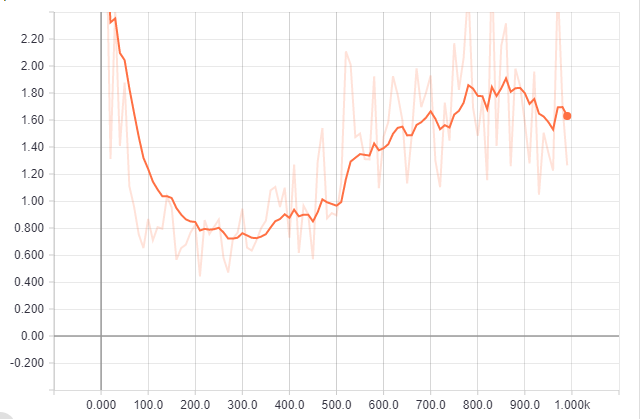
\includegraphics[width=\textwidth]{sections/experiments/overfitting}
	\caption{The development of the loss function on the validation set over the training.
	shows clear signs of overfitting. Smoothed to make the trend more clear}
	\label{fig:overfitting}
\end{figure}

\subsection{Measurements}

\begin{figure}
	\centering
	
	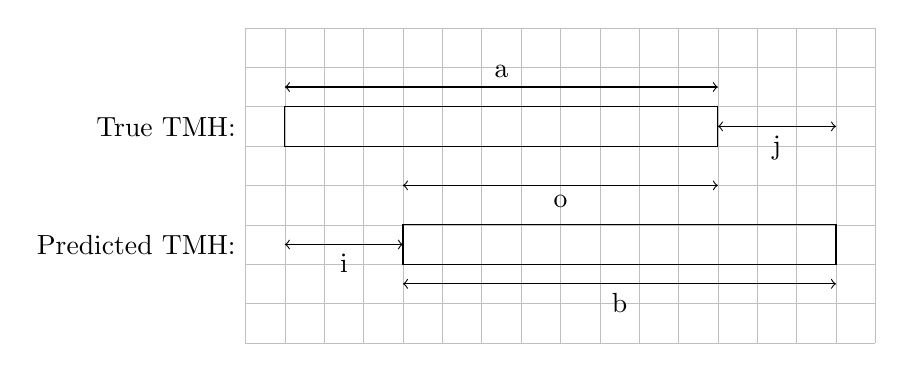
\begin{tikzpicture}[]
	\draw[step=0.5cm,very thin,color=lightgray] (0,-1) grid (8,3);
	
	\draw[] (0.5,1.5) rectangle (6,2);
	\node at (-0,1.5) [anchor=south east] {True TMH:};
	\draw[<->] (6,1.75) -- (7.5,1.75) node[pos=0.5, below]{j};
	\draw[<->] (0.5,2.25) -- (6,2.25) node[pos=0.5, above]{a};
	
	\draw[] (2,0) rectangle (7.5,0.5);
	\node at (-0,0) [anchor=south east] {Predicted TMH:};
	\draw[<->] (0.5,0.25) -- (2,0.25) node[pos=0.5, below]{i};
	\draw[<->] (2,-0.25) -- (7.5,-0.25) node[pos=0.5, below]{b};
	
	\draw[<->] (2,1) -- (6,1) node[pos=0.5, below]{o};
	\end{tikzpicture}
	
	\caption{Illustrations of used measurements in comparison of \glspl{tmh}. a is the length of true \gls{tmh},
		b is the length of the predicted \gls{tmh}, i is the difference in the start position, j is the difference
		in the end posetion and o is the length of the overlap.}
	\label{fig:thm_measurements}
\end{figure}

To evaluate the model some measure for the performance of the model have to be chosen.
I have chosen three different types of measurements that have three different purposes.
The loss function used in training of step 1 assigns a loss to each position with a 
wrong predicted class and the optimiser then tries to minimize this loss. 
Since the loss is calculated from each position, it seems apparent to also use a 
position based measurement. Especially to measure the performance of step 1.
This type of measurement does not see a \gls{tmh} as a single thing and can therefore
not say anything about the number of \glspl{tmh}. It is therefore also interesting 
to have a measure for this. I have used two different types of measurements to do this, 
both of them counts a consecutive sequence of positions classified as \gls{tmh} as a single
prediction. The purpose of step 1 was to identify regions with \glspl{tmh}.
The second measurement type's purpose is therefore to measure if a prediction of a 
\gls{tmh} is in the right region, this is done by finding the length of the overlap 
between the predicted \gls{tmh} and the true \gls{tmh}, denoted as $o$ in Figure 
\ref{fig:thm_measurements}, the length is then compared 
to the longest of the two \gls{tmh}. The predicted \gls{tmh} is counted as a correct prediction
if the ratio is larger than a certain value. This condition as an equation becomes:

\begin{equation}
	\frac{o}{\max(a, b)} \geq x
\end{equation}

Where $o$ is the length of the overlap, $a$ and $b$ is the length of the true \gls{tmh}
and the predicted \gls{tmh} respectively and $x$ is the minimum overlap ratio.
I have done this with different values to see how precise the predicted regions is. 

The last measurement type is intended to measure step 3. The purpose of
this step was to adjust the endpoints of predicted \glspl{tmh}, this measurement 
therefore looks at endpoints and counts a predicted \gls{tmh} as correct if both endpoints 
is within a certain number of positions of the true endpoints. 
As an equation this becomes:

\begin{equation}
	i \leq y \wedge j \leq y
\end{equation}

Where $i$ is the length between the start of the true \gls{tmh} and the predicted \gls{tmh},
$j$ is the length between the end of the two \gls{tmh} and $y$ is the maximum length these
differences can be. This is again done with 
different values for the allowed difference of endpoints. 

These two measurement types is derived from one of the measurement they use in TMSEG,
which is a combination of the two where the overlap have to be at least 50\% and the 
endpoints have to be within 5 positions of the true endpoints for a prediction to be counted
as correct. I have also used this measurement to be able to compare to the result they get 
there. 

For each condition for when a predicted \gls{tmh} is correct, precision and recall is calculated.
Precision is the percentages of the predicted \glspl{tmh} that is correct and recall is the 
percentages of true \glspl{tmh} that was correct predicted. Calculated the same way as in TMSEG:

\begin{align*}
	\text{Precision} &= \frac{\text{\# of correctly predicted TMHs}}{\text{\# of predicted TMHs}} * 100 \\
	\text{Recall} &= \frac{\text{\# of correctly predicted TMHs}}{\text{\# of true TMHs}} * 100
\end{align*}



% Sammenlign resultater mellem experimenterne og mellem andre modeller
% Kan vi se noget interressant i hvordan weights ser ud? 
\section{Evaluation}

\subsection{Results}

\begin{table}
	\centering 
	\begin{tabular}{l|c|c}
		Model & Precision & Recall \\ \hline
		Step1 w/o PSSMs & $81 \pm 0$ & $83 \pm 0$ \\
		Step1 w PSSMs & $81 \pm 0$ & $83 \pm 0$ \\
		Step2 w/o PSSMs & $81 \pm 0$ & $82 \pm 0$ \\
		Step2 w PSSMs & $81 \pm 0$ & $82 \pm 0$ \\
		Step3 w/o PSSMs & $73 \pm 0$ & $84 \pm 0$ \\
		Step3 w PSSMs & $73 \pm 0$ & $84 \pm 0$ \\
		HMM & $72 \pm 0$ & $31 \pm 0$ \\
	\end{tabular}
	\caption{Precision and recall for the position based measurement.}
	\label{tab:char}
\end{table}

The precision and recall for the position based measurement is shown in 
Table \ref{tab:char}. The model gives a moderately improvement to precision
in comparison with the \gls{hmm} and a massively improvement to recall.
Step 2 and 3 does almost nothing for the result. This is because the changes
they do is only a tiny part of all positions and therefore have little to 
no impact on the result of this measurement. 

\begin{table}
	\centering 
	\begin{subtable}[]{\textwidth}
		\begin{tabular}{l|c|c|c|c|c|c|c|c} 
			Model & \multicolumn{2}{|c}{10\%}& \multicolumn{2}{|c}{25\%}& \multicolumn{2}{|c}{50\%}& \multicolumn{2}{|c}{75\%}\\ 
			& Precis & Recall & Precis & Recall & Precis & Recall & Precis & Recall \\ \hline 
			Step 1 & $ 89 \pm 1 $ & $ 92 \pm 2 $ & $ 88 \pm 2 $ & $ 90 \pm 2 $ & $ 81 \pm 3 $ & $ 84 \pm 3 $ & $ 62 \pm 3 $ & $ 63 \pm 4 $ \\ 
			w PSSMs& $ 89 \pm 1 $ & $ 92 \pm 2 $ & $ 88 \pm 2 $ & $ 90 \pm 2 $ & $ 81 \pm 3 $ & $ 84 \pm 3 $ & $ 62 \pm 3 $ & $ 63 \pm 4 $ \\
			Step 2 & $ 92 \pm 1 $ & $ 94 \pm 2 $ & $ 92 \pm 1 $ & $ 94 \pm 2 $ & $ 85 \pm 2 $ & $ 87 \pm 2 $ & $ 64 \pm 3 $ & $ 65 \pm 3 $ \\ 
			w PSSMs& $ 92 \pm 1 $ & $ 94 \pm 2 $ & $ 92 \pm 1 $ & $ 94 \pm 2 $ & $ 85 \pm 2 $ & $ 87 \pm 2 $ & $ 64 \pm 3 $ & $ 65 \pm 3 $ \\ 
			Step 3 & $ 92 \pm 1 $ & $ 92 \pm 2 $ & $ 91 \pm 1 $ & $ 91 \pm 2 $ & $ 80 \pm 2 $ & $ 80 \pm 3 $ & $ 42 \pm 4 $ & $ 42 \pm 4 $ \\
			w PSSMs& $ 92 \pm 1 $ & $ 92 \pm 2 $ & $ 91 \pm 1 $ & $ 91 \pm 2 $ & $ 80 \pm 2 $ & $ 80 \pm 3 $ & $ 42 \pm 4 $ & $ 42 \pm 4 $ \\  
		\end{tabular}
		\caption{Precision and recall for 10\%, 25\%, 50\% and 75\% overlap of true \gls{tmh} and predicted \gls{tmh}.}
		\label{tab:overlap}
	\end{subtable}
	
	\begin{subtable}[]{\textwidth}
		\begin{tabular}{l|c|c|c|c|c|c|c|c} 
			Model & \multicolumn{2}{|c}{Below 10}& \multicolumn{2}{|c}{Below 5}& \multicolumn{2}{|c}{Below 2}& \multicolumn{2}{|c}{Equal 0}\\ 
			& Precis & Recall & Precis & Recall & Precis & Recall & Precis & Recall \\ \hline 
			Step 1 & $ 80 \pm 3 $ & $ 82 \pm 3 $ & $ 64 \pm 3 $ & $ 66 \pm 3 $ & $ 26 \pm 3 $ & $ 27 \pm 4 $ & $  2 \pm 1 $ & $  2 \pm 1 $ \\ 
			w PSSMs& $ 80 \pm 3 $ & $ 82 \pm 3 $ & $ 64 \pm 3 $ & $ 66 \pm 3 $ & $ 26 \pm 3 $ & $ 27 \pm 4 $ & $  2 \pm 1 $ & $  2 \pm 1 $ \\
			Step 2 & $ 84 \pm 2 $ & $ 86 \pm 2 $ & $ 67 \pm 3 $ & $ 69 \pm 3 $ & $ 27 \pm 3 $ & $ 28 \pm 3 $ & $  2 \pm 1 $ & $  2 \pm 1 $ \\ 
			w PSSMs& $ 84 \pm 2 $ & $ 86 \pm 2 $ & $ 67 \pm 3 $ & $ 69 \pm 3 $ & $ 27 \pm 3 $ & $ 28 \pm 3 $ & $  2 \pm 1 $ & $  2 \pm 1 $ \\
			Step 3 & $ 77 \pm 2 $ & $ 77 \pm 3 $ & $ 49 \pm 3 $ & $ 49 \pm 4 $ & $ 18 \pm 2 $ & $ 18 \pm 2 $ & $  1 \pm 1 $ & $  1 \pm 1 $ \\ 
			w PSSMs& $ 77 \pm 2 $ & $ 77 \pm 3 $ & $ 49 \pm 3 $ & $ 49 \pm 4 $ & $ 18 \pm 2 $ & $ 18 \pm 2 $ & $  1 \pm 1 $ & $  1 \pm 1 $ \\
		\end{tabular}
		\caption{Precision and recall for endpoints difference between true 
			\gls{tmh} and predicted \gls{tmh} below or equal to 10, 5, 2 and 0.}
		\label{tab:endpoint}
	\end{subtable}
	\caption{Results of different overlap ratios and endpoints differences comparing the different layers of the model.
	Error rates is specified as the standard deviation of the multiple runs of the experiments.}
	\label{tab:step_compare}
\end{table}

Table \ref{tab:step_compare} contains the result for different measurements 
comparing the steps in the model. Unsurprising goes both the precision and the 
recall down when the requirement for the predictions gets stricter. In 
Table \ref{tab:overlap} can it be seen that the difference between $10\%$ and $25\%$
overlap is very small and within one standard deviation from each other, 
this is implying to that if the model have made a prediction it has more than 
$25\%$ or less than $10\%$ overlap with a true \gls{tmh}.
Table \ref{tab:endpoint} shows that the changing the endpoint requirement a little 
gives a big difference in the result, from a precision on $84 \pm 2$ for an endpoints 
difference up to $10$ to a precision on $2 \pm 1$ for no endpoints difference.
Both precision and recall is very low if the requirement for a predicted \gls{tmh}
to be correct is that there is no difference in the endpoints, ie. the prediction 
is $100\%$ correct, which means there are almost no $100\%$ correct predictions.
From both measurement types can it be seen that step 2 helps a lot on especial 
the precision. This is because it removes a lot of small \glspl{tmh} from the 
prediction that does not correspond to real \glspl{tmh}, these small predicted 
\glspl{tmh} was lowering the precision but don't have much impact on the recall.
The results from step 3 is not very good, it doesn't change the result for 
$10\%$ and $25\%$ overlap, but it is still slightly worse than step 2. 
For $50\%$ overlap and endpoints difference below 5 and 10, it considerable lowers
both precision and recall and for $75\%$ overlap and endpoints difference below 
2, step 3 almost halve the results. The increasing impact step 3 has on the 
result as the requirement for the predictions gets stricter, is because step 3 
can only move the endpoints 6 positions and 6 positions don't have much impact 
if a prediction only has to have $10\%$ overlap but have a very large impact 
if the endpoint difference has to be below 2. 
Looking closer at the prediction from step 3 used to adjust the endpoints, it 
seems to give the same probability for every segment. The probabilities only
differs in the fifth decimal point and looks more like rounding inaccuracy
than predictions. The model does not seem to be able to learn any meaningful
thing from the input and have minimized the loss by always predicting the 
distribution of the labels in the training data. 
This failure to learn the patterns in the input data to accurately predict
the start end end of \glspl{tmh} could be because patterns is too complex or 
indistinct to learn with the size of the dataset or with the layout of the 
model.

\begin{table}
	\centering 
	\begin{tabular}{l|c|c} 
		Model & Precision & Recall \\ \hline
		Step 1 & $64 \pm 3$ & $66 \pm 4$ \\ 
		w PSSMs& $64 \pm 3$ & $66 \pm 4$ \\
		Step 2 & $67 \pm 3$ & $69 \pm 3$ \\ 
		w PSSMs& $67 \pm 3$ & $69 \pm 3$ \\
		Step 3 & $49 \pm 3$ & $49 \pm 4$ \\
		w PSSMs& $49 \pm 3$ & $49 \pm 4$ \\
		HMM   & $34 \pm 0$ & $13 \pm 0$ \\ 
		TMSEG\cite{tmseg} & $87 \pm 3$ & $84 \pm 3$
	\end{tabular}
    \caption{Precision and recall for 50\% overlap and endpoints difference below 5.}
	\label{tab:pr50}
\end{table}

In Table \ref{tab:pr50} is the precision and recall from using the same 
measurement as used by TMSEG. It also shows how the model compares with 
other models. TMSEG is a lot better at both precision and recall, 
but the model is a big improvement to the simple \gls{hmm}
based model. 

\subsection{Running time}
\label{sec:time}

%Inference time for step 1: 1.6142690181732178
%Inference time for step 2: 0.0045070648193359375
%Inference time for step 3: 2.752535581588745
%Training time for step 1: 800.2764098644257
%Training time for step 3: 1267.4366292953491

%Training time: 0.049510955810546875
%Decoding time: 0.8011248111724854

\begin{table}
	\centering 
	\begin{tabular}{l|c|c} 
		Model & Training & Inference \\ \hline
		Step 1 & 800 & 1.61 \\ 
		Step 2 & - & 0.005 \\ 
		Step 3 & 1267 & 2.75 \\
		HMM   & 0.0495 & 0.80
	\end{tabular}
	\caption{Training and inference timings for the different steps 
		and for a \gls{hmm}. All numbers in seconds. Training was done
		on the three first subset and inference was done on the last.}
	\label{tab:time}
\end{table}

Table \ref{tab:time} contains timings of the training and inference of each 
step of the model and of the simple \gls{hmm}. It takes a lot longer to train 
step 1 and step 3 than it does to use them to inference. 
It takes a lot longer to use the \gls{hmm} for inference than it does to train
it but it is still faster than the \glspl{lstm}. Since training only have to be
done once and the trained model can be saved and used later, the slow training 
time is not a huge disadvantages in comparison with other models. The inference
time is more important, because that is the time that is relevant if the model 
was to be used, and while it is also slower than the \gls{hmm} for inference,
it is not much slower.

\subsection{Discussion}
% What have we achieved? 
% Further work for it to be even better. 

%\subsection{Learning what the Model has Learned}
% Can we learn something from what the model has learn. By somehow visualising the weight matrices we can
% se what the model has found to be importen and sometimes something interresting aboubt the problem can be learned

\subsection{Further Work}
The model does not predict the topology of the structure, i.e. which 
non-\gls{tmh} parts are inside the membrane and which parts are outside.
Step 4 of TMSEG is the part of their model that does this and if I had more
time was this the first improvement I would add to this model.
Other interesting things to take a look at is other classes in the 
structure like signal peptides and reentrant loops. 
The model was also only trained to look at \glspl{tmp} and not 
soluble proteins and can therefore not be used to discriminate 
between those. This is something TMSEG does really well and 
something I would have looked at if I had more time.
For a more distant goal it could be interesting to examine other \gls{rnn}
architectures to see if others was more suitable to the problem and
if it was possible to improve the result by also using feature extraction.






\section{Conclusion}

\printbibliography

\end{document}}